\chapter{Annotation guidlines}

- Manually annotated datasets are essential to build and evaluate argumentation 
mining models. \\
- high quality dataset annotation requires that annotators are well trained in the task at hand \\
- data should be consistently annotated between indepedently working annotators \\
- having quality labelled data is a necessary foundation to build machine learning 
models \\
- to ensure annotators are understand the assigment and are able to complete 
the annotation task successfully, good annotation guidelines are required \\
- during the annotation of data described in this thesis  
annotators had to do a test annotation before the real one, 
discuss differently annotated examples until resolution, and redo annotation of examples
where there was no consensus available  \\
- this chapter shows the annotation guidelines for \begin{enumerate*}
\item microstructures (\ref{sec:microstructure_annotation_appendix}), 
\item argumentative segments,
\item claim formalizations and
\item argument comment relationship pairs
\end{enumerate*}

\section{Microstructure annotation guidelines}
\label{sec:microstructure_annotation_appendix}

\noindent - Microstructures represent logically structured argumentative claims
\citep{boltuzic2017toward}. \\
- One can expresses logically equivalent claims in language \\
- To limit the language variation microstructures were designed to translate
expression rich phrases to be translated to a restricted language to allow for
easier inference \\
- microstructures  consist of domain specific concepts, 
connected through a finite set of argumentative relations, expressed using 
a certain modality \\
- microstructure annotation proceduced the microstructures data (
see item element in \ref{item:microstructures_dataset})\\

\newpage
\subsection{Cheat sheet}

\begin{minted}{microstructure_lexer.py:MicroStructureLexer -x}
viewpoint_1(
	viewpoint_2[holder](
		relation_1([quantity_1] concept_1, [quantity_2] concept_2)
	)
)

concept_1 = concept OR relation_2(concept_3, concept_4)
concept_2 = concept OR relation_3(concept_5, concept_6)

\end{minted}

\noindent \textbf{Viewpoints} \\
- Believes, Approves, Disapproves, Desires

\begin{minted}{microstructure_lexer.py:MicroStructureLexer -x}
viewpoint_1(
	relation_1(relation_2(concept_3, concept_4), concept_2)
)
\end{minted}

\noindent \textbf{Relations} (grayed columns indicate dual meaning between relations in each row)

\begin{table}[!htb]
\begin{tabular}{|c c c c c c|}
\hline
\cellcolor{gray!25} \texttt{promotes} & \cellcolor{gray!25}\texttt{allow} & \texttt{purpose} & \texttt{equal} & \cellcolor{gray!25}\texttt{entails}     & \texttt{has\_associated} \\
\cellcolor{gray!25} \texttt{suppress} & \cellcolor{gray!25}\texttt{deny}  &         &       & \cellcolor{gray!25}\texttt{contradicts} &  \\
\hline
\end{tabular}
\end{table}

\noindent \textbf{Negation} (use with relations)
Use with relation in front (\texttt{not\_promotes}, \texttt{not\_suppress}, \dots) \\
 
\noindent \textbf{Quantities} (use with concepts) \\
Some, All, Minority, Majority \\
          
\noindent \textbf{Concepts} 
\footnote{\url{https://docs.google.com/document/d/1ETobyCA4mpMmml1HXyxD7IG67EzrNK7W_2gzaIN0k_k/edit}} \\

\noindent \textbf{Quality} $\in [1, 5]$ \\
 
\noindent \textbf{Stance} $ \in {-2, -1, 0, 1, 2}$ \\

\pagebreak

\subsection{Task description}

In this task we annotate argumentative sentences/claims and represent them
using a logical generative grammar language, as well as a stance. The
argumentative sentences are paraphrases of debate post excerpts. We will
provide you with the original post, as the argumentative sentences provided
might not be enough to fully understand the meaning. 
The language has a set of syntactic rules, which need to be respected. The
syntax of your solutions will be checked as you annotate the document. 
An example sentence will look like:
\noindent\begin{tabular}{@{}lp{0.8\columnwidth}}
(ex. 1) & \textit{Homosexual marriage can not truly be a marriage.}
\end{tabular} \vspace{0.4cm}

\noindent We want to translate this to the form of: 

\begin{tabular}{@{}m{1.5cm}  m{4.5cm}}
(ex. 1) &  \begin{minted}{microstructure_lexer.py:MicroStructureLexer -x}
believes(
    contradicts(homosexual marriage, marriage)
)
\end{minted}
\end{tabular}

In this context, we call homosexual marriage and marriage concepts. The element
contradicts is a relation between the concepts. Believes is a viewpoint that
depicts the author's perspective. See more on concepts, relations and
viewpoints in the language description section below. 

Good practice when creating these annotations is attempting to read them back
in natural language. In this case, we get: I believe that homosexual marriage
is not marriage.  If we compare this to the original sentence, we see that it
captures the essence of the example sentence (ex. 1). The wording is lost,
which can mean a lot sometimes (reading between the lines), but this is
something we’re OK with.

\subsection{Language description}

As said, we annotate:
\begin{itemize}
\item Concepts
\item Relations between concepts
\item Viewpoints
\end{itemize}

\subsubsection{Concepts}

Concepts are noun phrases mentioned when discussing a topic. We provide a set
of concepts that we have previously identified for the ``gay rights'' topic\footnote{
Concepts available at 
\url{https://docs.google.com/document/d/1ETobyCA4mpMmml1HXyxD7IG67EzrNK7W_2gzaIN0k_k/edit?usp=sharing}
}
Some concepts are tab-shifted, which you can disregard, some have
slashes between them (i.e. \texttt{heterosexual marriage} / \texttt{traditional marriage}); we
consider these synonyms, please choose the first one. Your task is to search
through this list and find appropriate concepts (as close concept as possible)
mentioned in the input sentence and associate the appropriate relations between
them. Some example concepts: \texttt{procreation}, \texttt{reproduction}, \texttt{adoption}, \texttt{homosexual}
\texttt{adoption}, \texttt{have children}, \texttt{gay people}. 
If you feel you need to use a concept not
in the list, please contact us with the example. Another case would be where a
concept might be implicit, in the sentence: \textit{Allow gay marriages}, we recognize
the relation \texttt{allow} (explained in relations below) and the concept \texttt{gay marriages}
(argument B for relation \texttt{allow}).  We don’t know what the principle is, but from
the topic we know the state can allow gay marriages, therefore we can translate
the sentence as: \texttt{allow(state, gay marriage).}

\subsubsection{Quantity}

Each concept can be expressed with quantity. Quantities allowed are:
\begin{itemize}
\item Some 
\item All
\item Minority
\item Majority
\end{itemize}

\begin{table}[!htb]
\begin{tabular}{@{}m{1.5cm} m{5cm} m{8cm}}
\toprule
Example & Sentence & Microstructure \\
\midrule
(ex. 2.a) & Some people promote gay marriages. & 
\begin{minted}{microstructure_lexer.py:MicroStructureLexer -x}
believes(
  promote([some]people, gay marriage)
) 
\end{minted}
\\
(ex. 2.b) &Democracy helps the majority of people. &
\begin{minted}{microstructure_lexer.py:MicroStructureLexer -x}
believes( 
  promote(democracy, [majority] people)
)
\end{minted} 
\\
\bottomrule
\end{tabular}
\end{table}

\subsubsection{Relations}

Relations are connections between concepts. Relations are not domain-bound (one
can use them outside of gay marriages), while concepts are tied to domain 
(\texttt{gay marriages} in this case). Relations are verb phrases. 
Possible relations are:

\begin{footnotesize}
\begin{tabular}{lp{5cm}p{2.5cm}p{3cm}}
\toprule
Relation & Explanation & Argument A & Argument B \\
\midrule
\texttt{promotes(A, B)} & 
\makecell[cl]{
\textbf{A} promotes / fosters / \\
brings about / leads \\ 
/ forces / advances \\
/ increases /encourages \\
/ boosts / increases \\
the likelihood of / causes \textbf{B}  \\ \\
``Soft causation'' \\\\
\href{https://framenet2.icsi.berkeley.edu/fnReports/data/frameIndex.xml?frame=Cause_change_of_position_on_a_scale}{FrameNet link} 
}
& 
Agent (which promotes) & 
Attribute (what gets promoted) \\
\midrule
\texttt{suppress(A, B)} & 
\makecell[cl]{
\textbf{A} suppresses / decreases \\ 
likelihood / smothers / \\
represses / puts down / \\
vaniquishes \textbf{B} 
}
&
Agent (which suppresses) & 
Attribute (what gets suppressed)
\\
\midrule
\texttt{allow(A, B)} & 
\makecell[cl]{
Principle \textbf{A} \\ 
allows / approves / \\
licenses \textbf{B} \\\\
\href{https://framenet2.icsi.berkeley.edu/fnReports/data/frameIndex.xml?frame=Prohibiting_or_licensing}{FrameNet link}
} & 
Principle
& 
State of affairs \\
\midrule
\texttt{deny(A, B)} & 
\makecell[cl]{
Priciple \textbf{A} \\
denies / disallows /
bans \textbf{B} } & 
Principle & 
State of affairs\\
\midrule
\texttt{entails(A, B)} & 
\makecell[cl]{
State of affairs \textbf{A} \\
necessarily, per definition \\
or causally, makes \textbf{B} true \\\\
Proposition \textbf{B} has \\
support \textbf{A} \\\\
\href{https://framenet2.icsi.berkeley.edu/fnReports/data/frameIndex.xml?frame=Evidence}
{FrameNet link}
}
& State of affairs & Implication \\
\midrule
\texttt{contradicts(A, B)} & 
\makecell[cl]{
State of affairs \textbf{A} \\
makes \textbf{B} not true}
& State of affairs & Contradiction \\
\midrule
\texttt{purpose(A, B)} & 
\makecell[cl]{The purpose of \textbf{A} is \textbf{B} \\\\
\href{https://framenet2.icsi.berkeley.edu/fnReports/data/frameIndex.xml?frame=Purpose
}{FrameNet link}
} & Agent & Goal \\
\midrule
\texttt{has\_associated(A, B)} &
\makecell[cl]{
\textbf{A} has properties affected by \\
the existence of \textbf{B} \\\\
\href{https://framenet2.icsi.berkeley.edu/fnReports/data/frameIndex.xml?frame=Membership
}
{Similar FrameNet definition} 
} & Group & Member \\
\midrule
\texttt{equal(A, B)} & \textbf{A} is equal to \textbf{B} & Concept \textbf{A} & Concept \textbf{B} \\
\bottomrule
\end{tabular}
% \caption{Relation definition table}
% \label{tab:relation_definition}
% \end{table}
\end{footnotesize}

\subsubsection{Negation}
%TODO proper references in table rows

Relations can be negated to indicate opposite meaning. Notice how example $3.a$
is not saying it is suppressing, but just denied promoting. Example $3.b$ also can’t
use contradicts since being happy does not imply you are not rich, but it does
not imply you are.

\begin{footnotesize}
\begin{tabular}{@{}m{1.5cm} m{5cm} m{8cm}}
\toprule
Example & Sentence & Microstructure \\
\midrule
(ex. $3.a$) & \textit{Marijuana does not help cure cancer. } & 
\begin{minted}{microstructure_lexer.py:MicroStructureLexer -x}
believes(
  not_promotes(marijuana, cure cancer)
)
\end{minted}
\\
(ex. 3.b) & \textit{If you are happy, doesn’t mean you’re rich.} 
 &
\begin{minted}{microstructure_lexer.py:MicroStructureLexer -x}
believes(
  not_entails(feel happy, be rich)
)
\end{minted} 
\\
\bottomrule
\end{tabular}
\end{footnotesize}

\subsubsection{Nested Relations}

Relations can be nested within each other. Each relation takes two arguments.
An argument can be another relation or a concept. Make sure you are correct
with closing the opened braces. 

\begin{footnotesize}
\begin{tabular}{@{}m{1.5cm} m{5cm} m{8cm}}
\toprule
Example & Sentence & Microstructure \\
\midrule
(ex. $4.a$) & \textit{I think allowing gay marriages promotes freedom. } & 
\begin{minted}{microstructure_lexer.py:MicroStructureLexer -x}
believes(promotes(
  allow(state, gay marriage), freedom
  )
)
\end{minted}
\\
(ex. 4.b) & \textit{The purpose of life is to allow having freedom.} 
 &
\begin{minted}{microstructure_lexer.py:MicroStructureLexer -x}
believes(
  purpose(life, 
    allow(state, freedom)
  )
)
\end{minted} 
\\
(ex. 4.c) & \textit{It’s the same thing to allow gay marriages or heterosexual marriages.} & 
\begin{minted}{microstructure_lexer.py:MicroStructureLexer -x}
believes(
  equal(
    allow(state, gay marriage), 
    allow(state, heterosexual marriage)
  )
)
\end{minted}
\\
\bottomrule
\end{tabular}
\end{footnotesize}

\subsubsection{Viewpoints}

Viewpoints reflect whether the a viewpoint holder thinks the claim is believed
(fact), desired (policy), or considered right/wrong (value judgement). When not
mentioned, the claim holder is considered to be the author of the argumentative
sentence. If not, one needs to annotate the claim holder next to the viewpoint
type (\textit{I believe the Bible states}, \textit{I think the state of Florida should}), which
we call second-level viewpoints. Second-level viewpoints are annotated together
with a concept, for example: "\textit{I saw that the Bible states: It should be
allowed}" corresponds to "\texttt{believes(believes[Bible]...))}".
Possible viewpoints are \\

\begin{tabular}{l p{7cm} p{6cm}}
\toprule
Viewpoint & Description & Example \\
\midrule
\textbf{believes} & \textbf{A} believes / argues / thinks
that claim \textbf{C} is true & 
I believe people are mortal. \\
\midrule
\textbf{desires} & 
\textbf{A} believes / argues / thinks \textbf{C} 
should be true in the future or should remain true
& People should be nicer \\
\midrule
\textbf{approves} & 
\textbf{A} believes / argues / thinks \textbf{C} 
is morally / ethically right & Forgiving is bad \\
\midrule
\textbf{disapproves} & 
\textbf{A} believes / argues / thinks \textbf{C} 
is morally / ethically wrong & 
Drugs are bad.  \\
\bottomrule
\end{tabular} \\
% \label{tab:viewpoints}
% \caption{Viewpoints, their descriptions and examples of using specific viewpoints in claims}

\noindent Annotating a claim holder explicitly should be done like for sentence:

\begin{table}[h]
\begin{tabular}{@{}m{1.5cm} m{5cm} m{8cm}}
\toprule
Example & Sentence & Microstructure \\
\midrule
(ex. $5.a$) & \textit{I saw the Bible claims gay people are equal to straight people} & 
\begin{minted}{microstructure_lexer.py:MicroStructureLexer -x}
believes(
  believes[Bible](
    equal(gay people, straight people)
  )
)
\end{minted}
\\
\bottomrule
\end{tabular}
\label{tab:viewpoint_example}
\caption{Viewpoint claim annotation example}
\end{table}

\subsubsection{Stance}

Please annotate stance, which answers the question:
\textbf{Is the sentence pro-gay or not just by looking only at the offered claim} (not
the entire post context)? Stance $\in {-2, -1, 0, 1, 2}$.

\begin{table}[!htb]
\begin{tabular}{c p{10cm}}
\toprule
Stance Value & Explanation \\
\midrule
-2 & The author or the viewpoint of the second person is definitely against the
claim (explicitly states so). Any form of discrimination is seen as against.  \\
-1 & There is some implication that the author might be against gay rights  \\
0 & There is no stance towards gays, stance is bipolar \\
1 & Reverse of -1 \\
2 & Reverse of -2 \\
\bottomrule
\end{tabular}
\label{tab:stance}
\caption{Possible stance values with explanations}
\end{table}

\begin{table}[!htb]
\begin{tabular}{c p{10cm} r}
\toprule
Example & Claim & Stance \\
\midrule
(ex. $6.a$) &  I think allowing gay marriages promotes freedom. & 2 \\
(ex. $6.b$) & All people are equal. & 0 \\
(ex. $6.c$) & Allowing gay marriages will be the end of us all. &  -2 \\
(ex. $6.d$) & I would ban religious gay marriage. & -2 \\
(ex. $6.e$) & The Bible is against gay marriages & -2 \\
\bottomrule
\end{tabular}
\label{tab:stance_example}
\caption{Examples of stance for the gay marriages topic}
\end{table}

\subsubsection{Quality}

Evaluate your own logical claim transformation by inputting a number $\in [1, 5]$
rating how well does the proposed formalization suit what the person said?

\subsection{Technical instructions}

You will be provided with an excel spreadsheet with the posts and sentences.
Please notify us as soon as possible if you can’t use Excel - we can send you
the annotation in another format (Google spreadsheet, etc.). 

The goal is to fill up the E, F, G columns (logical representation, stance and
quality, highlighted in green) in the provided spreadsheet based on the
argumentative sentence in column D. Feel free to ignore columns A, and C (used
for internal tracking). Column B might be useful, if you can’t determine the
meaning in D. If you have problems or comments about an example, feel free to
add them in column H and raise questions with us -- we will be happy to
discuss! An example row will look like in table~\ref{tab:annotation_example}

\begin{table}[!htb]
\scriptsize
\begin{tabular}{|p{1.5cm} | p{2cm} | p{2cm} | p{2cm} | p{2cm} |c| c| c|}
\toprule
A & B & C & D & E & F & G & H \\
\midrule
POST ID & POST TEXT & SEGMENT ID & SENTENCE & LOGICAL REPRESENTATION
& STANCE & QUALITY & COMMENTS \\
\midrule
A75.data & 
Here we is the full text of the post. This will be relatively long.
This is divided into segments (argumentative sentences) that you then annotate. 
& 758 & 
The full text of the post will be relatively long.  
& \cellcolor{green!25} &  \cellcolor{green!25}& \cellcolor{green!25} & \cellcolor{green!25} \\
\bottomrule
\end{tabular}
\caption{Example excel sheet to annotate}
\label{tab:annotation_example}
\end{table}

A syntax checking script and your annotation is packaged into a zip file.  Your goal is to
fill column E in \texttt{annotation.xls}.

\subsubsection{Checking syntax correctness (optional)}

We provide a script to verify that your solutions are syntactically correct. 
You will need to install python and a python library xlrd. Make sure to install
\texttt{python 2.x}!

If you are not familiar with python, installing them on Windows is desribed in
\url{http://www.howtogeek.com/197947/how-to-install-python-on-windows/}
Xlrd is available to install from:
\url{http://www.lexicon.net/sjmachin/xlrd-0.6.1.win32.exe} 
To install it, you will need to Run-as-administrator. 
Please contact us if you have issues installing these. 
To help check correctness of your solution, we offer a python script that can
be run in two ways:

\begin{description}[style=multiline, labelwidth=1.5cm]
\item[\namedlabel{item:excel}{All}] Check all solutions in your excel spreadsheet
\item[\namedlabel{item:single_claim}{Single}] Check a single claim
\end{description}

\begin{figure}
	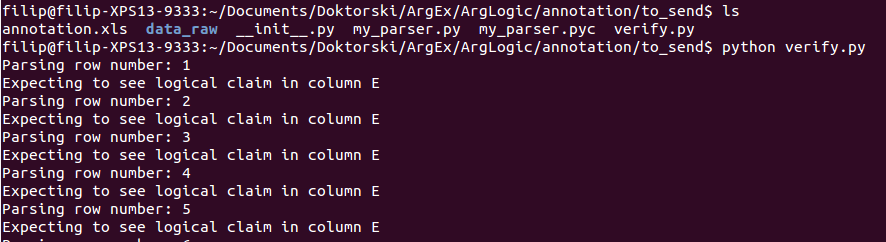
\includegraphics[scale=0.5]{struc_instructions_1.png}
	\caption{Expected output of running microstructure syntax check on entire file (\ref{item:excel}) mode}
	\label{fig:struc_instructions_all}
\end{figure}

\begin{figure}
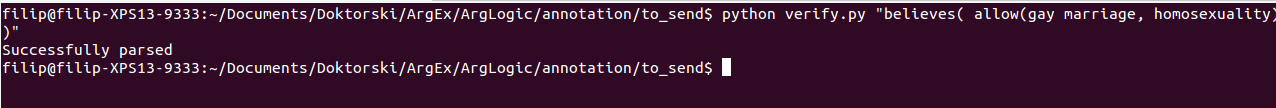
\includegraphics[scale=0.35]{struc_instructions_2.png}
	\caption{Expected output of running microstructure syntax check on a
	\label{fig:struc_instructions_2}
	single claim (\ref{item:single_claim} mode) }
\end{figure}

\noindent The script and your annotation is packaged into a zip available here. When you
unzip it, you should input your solutions in excel file \texttt{to\_send/annotation.xls}
To run it in \ref{item:excel} mode simply run \texttt{python verify.py} while
positioned in the \texttt{to\_send} directory using the command line (shown in
figure~\ref{fig:struc_instructions_all}) To run in \ref{item:single_claim}
mode, also position yourself in the \texttt{to\_send/} directory, but run as
shown in figure~\ref{fig:struc_instructions_2}.


\section{Claim segment annotation}
\label{sec:argseg_annotation}

Annotating claim segments from user comments splits the comment into claims. The
claims can be transformed into microstructures (as done to create the
microstructure dataset described in~\ref{item:microstructures_dataset}) or
formalized structures (as done to create the argument structure dataset
described in~\ref{item:structure_dataset}). Annotating segments involves
paraphrasing extracted segments to help streamline the annotation of segments
to structures. 

The task is to segment debate posts into claims. Each annotator gets a sheet in
a Google Sheets file with their name.  Column $C$ contains a user comment on
the topic of ``\textit{Should marijuana be legal}'' (MA).  The annotator needs
to carefully read the user comment, determine the stance of the comment along
with the explicit and implicit claims upon which the comment founds the
expressed stance. 

For each comment, the annotation involves:
\begin{enumerate}
\item extracting all argumentative segments of the comment as an atomic claim,
\item labeling the type of extracted segments, and
\item creating a paraphrase of the extracted segment.
\end{enumerate}
All argumentative segments should be copied to column $D$. 
Each extracted segment needs to be marked with an integer which denotes the
ordering of appearance in the post (segment $S1$, $S2$, $S3$, \dots)
All text belonging to segment $S1$ needs to be copied to column $D$, whereas
the original comment text needs to be edited to mark the segments belonging to 
the extracted segments. The beginning and end 
of the segment $Sx$ need to be marked with \texttt{<Sx>} and \texttt{</Sx>} respectively. 
Discontiguous segments are also allowed, they need to be marked with start and end tags
for each segment. Copying discontiguous segments is done by concatenating all 
instances in order of appearance. 
Column $E$ needs to contain the segment 
identifier ($S1$, $S2$, \dots). Please note that each start tag needs to be
paired with an end tag. 

\noindent Example 1: 

\begin{itemize}
  \item[] Comment: ``People are great, they have many virtues.''
  \item[] Segment $S1$: ``People are great''
  \item[] Segment $S2$: ``they have many virtues''
  \item[] Edited comment: ``\texttt{<S1>}People are great\texttt{</S1>},
  \texttt{<S2>}they have many virtues\texttt{</S2>}. ''
\end{itemize}

\noindent Example 2:
\begin{itemize}
\item[] Comment: ``People are smart and stupid.''
\item[] Segment $S1$: ``People are smart''
\item[] Segment $S2$: ``People are stupid''
\item[] Edited comment: ``\texttt{<S1><S2>}People are\texttt{</S2>} smart\texttt{</S1>}
and \texttt{<S2>}stupid\texttt{</S2>}''
\end{itemize}

\subsection*{Argumentative segment type}

The extracted segment needs to have a labelled segment type in column $F$ of
the Google sheets document. The segment needs to be classified according to two
taxonomies. First, the segment needs to be classified as either a 
\begin{enumerate}
\item fact --- statement that is true or untrue,
\item policy --- statement providing a solution or another series of questions in response to a fact,
\item value --- judgement, appraisal or evaluation. 
\end{enumerate}
Second, the segment needs to be labelled as either a 
\begin{enumerate}
\item assertion --- explicit statement or announcement or
\item rhetorical question --- question not expecting an answer. 
\end{enumerate}
More on facts, values and policies \citep{factvaluepolicy}.

\subsection*{Segment paraphrase annotation}

For each extracted segment, a paraphrase needs to be constructed. The paraphrase needs to
be assigned to column $G$ in spirit of the following principles:
\begin{itemize}
\item \textbf{Argumentativeness} -- Only argumentative text should be paraphrased; 
\item \textbf{Atomicity} -- A claim should convey a single thought; 
\item \textbf{Authority} -- Experts in claims from expert opinion should be made explicit in the paraphrase; 
\item \textbf{Brevity} -- Paraphrases should keep only the relevant argumentative content; 
\item \textbf{Canonicity} -- Canonical terms and phrases are preferred over idiomatic language;
\item \textbf{Contextuality} -- Claims should be paraphrased by considering their local and
topical context as well as their context;
\item \textbf{Declarativity} -- paraphrases should 
be in declarative form;
\item \textbf{Dereferencing} -- Pronouns and nominal  references
should be  resolved;  and
\item \textbf{Explicitness} -- Only explicitly stated
information should be paraphrased, and not whatever might be implied by the claim
\end{itemize}

\subsection*{Examples of segment annotation}

\begin{mydef}
By banning gay adoption, children in gay couple households have no legal status
should something happen to the parents, including death or serious illness.
The child cannot claim inheritances or other household assets in case of death.
If one parent dies, the second parent has no legal right to take custody or
care for the child.   A parent without legal right to a child cannot legally
register him/her for school.   Parents cannot put children on some health
insurance plans.   Parents cannot make medical decisions for the child.   * The
child has no claim to the social security or other insurance benefits of the
parent.   Gay couple parents without adoption rights do not benefit from the
generous tax deductions granted to heterosexual parents.
\end{mydef}

\noindent Extracted segments:
\begin{itemize}
\item[] \textbf{Segment1:} ``By banning gay adoption, children in gay couple
households have no legal status should something happen to the parents,
including death or serious illness.''
\item[] \textbf{Type}: Fact, assertion
\item[] \textbf{Paraphrase}: ``Children without a legal status are not
protected in case something happens to their parents''
\end{itemize}

\begin{itemize}[topsep=0.3cm]
\item[] \textbf{Segment2}: ``The child cannot claim inheritances or other household assets in case of death.''
\item[] \textbf{Type}: Fact, assertion
\item[] \textbf{Paraphrase}: ``Children without a legal status cannot claim
inheritance or other household assets in case of death.''
\end{itemize} 

\begin{itemize}[topsep=0.3cm]
\item[] \textbf{Segment3}: ``If one parent dies, the second parent has no legal
right to take custody or care for the child.''
\item[] \textbf{Type}: fact, assertion
\item[] \textbf{Paraphrase}: ``If one parent dies, the second parent has no legal
right to take custody or care for the child.'' (same)

\end{itemize}

\begin{itemize}[topsep=0.3cm]
\item[] \textbf{Segment4}: ``A parent without legal right to a child cannot
legally register him/her for school.''
\item[] \textbf{Type}: fact, assertion
\item[] \textbf{Paraphrase}: ``A parent without legal right to a child cannot
legally register him/her for school.'' (same)
\end{itemize}

\begin{itemize}[topsep=0.3cm]
\item[] \textbf{Segment5}: ``Parents cannot put children on some health insurance plans.''
\item[] \textbf{Type}: fact, assertion
\item[] \textbf{Paraphrase}: ``Parents cannot put children on some health insurance plans.'' (same)

\end{itemize}

\begin{itemize}[topsep=0.3cm]
\item[] \textbf{Segment6}: ``Parents cannot make medical decisions for the child.''
\item[] \textbf{Type}: fact, assertion
\item[] \textbf{Paraphrase}: ``Parents cannot make medical decisions for the child.''
\end{itemize}

\begin{itemize}[topsep=0.3cm]
\item[] \textbf{Segment7}: ``The child has no claim to the social security or
other insurance benefits of the parent''
\item[] \textbf{Type}: fact, assertion
\item[] \textbf{Paraphrase}: ``The child has no claim to the social security or
other insurance benefits of the parent''
\end{itemize}

\begin{itemize}[topsep=0.3cm]
\item[] \textbf{Segment8}: ``Gay couple parents without adoption rights do not
benefit from the generous tax deductions granted to heterosexual parents.''
\item[] \textbf{Type}: fact, assertion
\item[] \textbf{Paraphrase}: ``Unmarried gay parents cannot claim adoption rights
to benefit from tax deductions.''
\end{itemize}

\begin{mydef}
No it shouldnt be allowed. Marriage is when man and women get married. In the
Bible it says that its a sin for marrying your same gender and its a immoral
sin. Look at the animals they have one male and one female you dont see 2 male
horse with each other or any other animals. Look at the example animals make
learn from them.
\end{mydef}

\begin{itemize}[topsep=0.3cm]
\item[] \textbf{Segment1}: it shouldnt be allowed
\item[] \textbf{Type}: policy, assertion
\item[] \textbf{Paraphrase}: Gay marriage should not be allowed.
\end{itemize}

\begin{itemize}[topsep=0.3cm]
\item[] \textbf{Segment2}: Marriage is when man and women get married.
\item[] \textbf{Type}: fact, assertion
\item[] \textbf{Paraphrase}: Marriage is between a man and a woman.
\end{itemize}

\begin{itemize}[topsep=0.3cm]
\item[] \textbf{Segment3}: In the Bible it says that its a sin for marrying your same gender and its a immoral sin.
\item[] \textbf{Type}: fact, assertion
\item[] \textbf{Paraphrase}: According to the bible, same-sex marriage is immoral.
\end{itemize}

\begin{itemize}[topsep=0.3cm]
\item[] \textbf{Segment4}: Look at the animals they have one male and one female
\item[] \textbf{Type}: fact, assertion
\item[] \textbf{Paraphrase}: Animals of opposite sex pair up.
\end{itemize}

\begin{itemize}[topsep=0.3cm]
\item[] \textbf{Segment5}: you dont see 2 male horse with each other or any other animals
\item[] \textbf{Type}: fact, assertion
\item[] \textbf{Paraphrase}: Animals of same sex do not pair up.
\end{itemize}

\begin{itemize}[topsep=0.3cm]
\item[] \textbf{Segment6}: Look at the example animals make learn from them.
\item[] \textbf{Type}: policy, assertion
\item[] \textbf{Paraphrase}: We should learn from how animals behave.
\end{itemize}

\subsubsection*{Segment atomicity}

\begin{mydef}
I do not at all feel as God wants two men or two woman to be together, as he
has made each a man and a woman to combine and be together. However, it is our
constitutional right to make our own chices in America. What I believe should
be "exit only" is non of my business where people put things. As far as a legal
bond, we are considered "one nation under God" but , the goverment would make a
benifit from gay marriage, wether I a gree or not. Like I said we should have
the freedom to choose, we are Americans and our ancestors fought for our
freedom!!!!! Hey and I hope everyone is fighting to keep seatbelts a
choice,please keep fighting for our FREEDOM of choice!!!
\end{mydef}
This extracted segment expresses two separate ``thoughts''
\begin{itemize}
\item[] ``What I believe should be "exit only" is non of my business where people put
things.''
\end{itemize}
therefore it should be divided into two segments:
\begin{itemize}
\item[]  ``I believe should be "exit only"''
\item[] ``is non of my business where people put things''
\end{itemize}

\subsection*{Assuming too many implicit premises}

\begin{mydef}
I do not at all feel as God wants two men or two woman to be together, as he
has made each a man and a woman to combine and be together. However, it is our
constitutional right to make our own chices in America. What I believe should
be "exit only" is non of my business where people put things. As far as a legal
bond, we are considered "one nation under God" but , the goverment would make a
benifit from gay marriage, wether I a gree or not. Like I said we should have
the freedom to choose, we are Americans and our ancestors fought for our
freedom!!!!! Hey and I hope everyone is fighting to keep seatbelts a
choice,please keep fighting for our FREEDOM of choice!!!
\end{mydef}
The segment ``our ancestors fought for our freedom'' can be understood
such that the author believes that freedom refers to the freedom of choice.
This might be the case, but concluding so requires making assumptions based 
derived on implicit premises. 

\begin{itemize}
\item[] ``American ancestors fought for freedom to choose''
\end{itemize}
This paraphrase assumes ``freedom to choose''. But, the same segment can be
paraphrased not to include implicit knowledge and paraphrase in the following way 
(while also dereferencing the pronoun ``our'' to ``Americans''):
\begin{itemize}
\item[] ``Ancestors of current Americans fought for freedom of Americans.''
\end{itemize}

\subsection*{Reusing segment parts}

\begin{mydef}
As you say, "Marriage is something in particular." Its a legal union requiring
a license from a government office, not from a religious organization. That's
why gay people are fighting for "equal rights", not "equal rites."   For the
government to remain neutral on this issue, they need to stop denying gay
people the same rights as others to marry. As it is, the federal government is
anything but neutral. They deny over one thousand federal benefits to people
legally married in several states who happen to be of the same sex.
\end{mydef}
One candidate segment to extract would be:
\begin{itemize}
\item[] ``For the government to remain neutral on this issue, they need to stop
denying gay people the same rights as others to marry''
\end{itemize}
This segment actually contains three connected atomic segments (in paraphrased form):
\begin{itemize}
\item[] ``The government needs to remain neutral on this issue''
\item[] ``The government needs to stop denying gay people rights to marry''
\item[] ``Everyone but gay people have the rights to marry''
\end{itemize}


\begin{mydef}
This is the dictionary definition of marriage:   a.   the social institution
under which a man and woman establish their decision to live as husband and
wife by legal commitments, religious ceremonies, etc. Antonyms: separation.
b.   a similar institution involving partners of the same gender: gay marriage.
Antonyms: separation.   2.   the state, condition, or relationship of being
married; wedlock: a happy marriage. Synonyms: matrimony. Antonyms: single life,
bachelorhood, spinsterhood, singleness; separation.   3.   the legal or
religious ceremony that formalizes the decision of two people to live as a
married couple, including the accompanying social festivities: to officiate at
a marriage. Synonyms: nuptials, marriage ceremony, wedding. Antonyms: divorce,
annulment.   4.   a relationship in which two people have pledged themselves to
each other in the manner of a husband and wife, without legal sanction: trial
marriage.   5.   any close or intimate association or union: the marriage of
words and music in a hit song. Synonyms: blend, merger, unity, oneness;
alliance, confederation. Antonyms: separation, division, disunion, schism.
There is no mention of the reason for marriage being to Pro-create, the only
reason people should get married should be because they love each other and if
two Gay people love each other they should be allowed to marry. You can
Pro-create without getting married and I know many straight married people who
dont have Children they married because they loved each other not to have
children and Gay people should be allowed this right as well
\end{mydef}
Segment ``many straight married people who dont have Children they married
because they loved each other not to have children''
can be divided into three atomic segments:
\begin{itemize}
\item[] ``many straight married people who don't have Children''
\item[] ``many people married because they loved each other''
\item[] ``many people married not to have children''
\end{itemize}

\subsection*{Recognizing value segments}

Value segments often involve explicitly judging the value of an object.
Sometimes, the judgement can be made implicitly, but seeing explicit 
expressions should be preffered. For example: 
``People argue Gay marriage will lead to and allow
nontraditional families.'' is a factual statement, because 
the author expresses his views of public opinion. If the author expressed
his personal view like ``gay marriages lead to nontraditional families''
this could be considered a value statement, with the key part being
the word ``nontraditional'' which expresses negativity towards ``gay marriages''.
Whether there is a another view holder can influence the segment type. 
The segment ``The bible says Gay rights are immoral'' is considered a factual statement, 
whereas the segment ``Gay rights are immoral'' is considered to be a 
value segment since the segment is attributed to the author. 

